\documentclass[dvipdfmx,12pt]{beamer}
\usepackage{bxdpx-beamer}
\usepackage{pxjahyper}
\usepackage{tikz}
\usepackage{here}
\usepackage{graphicx}
\renewcommand{\kanjifamilydefault}{\gtdefault}

\usepackage{amsmath}
\usepackage{amsfonts}
\usepackage{amssymb}
\usepackage{color}
\usepackage{tcolorbox}
\usepackage{forest}
\usepackage{ascmac}
\usepackage{fancybox}
\usetikzlibrary{arrows.meta}
\usetikzlibrary{positioning}

\usetheme{metropolis}  

% blockのスタイルをカスタマイズ
\setbeamercolor{block title}{bg=blue!30,fg=black} % タイトルの背景色とテキストの色
\setbeamercolor{block body}{bg=blue!10,fg=black} % ボディの背景色とテキストの色

\usepackage[usetype1]{uline--}

\title{第3回MPC勉強会}
\author{鶴原康太}

\begin{document}

    \frame{\maketitle}

    \begin{frame}{今回の目標}
        \begin{equation*}
            -\frac{\partial V}{\partial t}\left(x,t\right) = \min _u H\left(x, u, \left( \frac{\partial V}{\partial x} \right)^T\left(x, t\right), t \right)
        \end{equation*}
    \end{frame}

    \begin{frame}{現在位置}
        \begin{columns}
            \begin{column}{.5\textwidth}
                \begin{itemize}
                    \item \colorbox{yellow}{復習}
                    \item 動的計画法
                    \item HJB方程式
                    \item 最小原理
                    \item MPC導入
                \end{itemize}
            \end{column}
    
            \begin{column}{.5\textwidth}
                今までの内容覚えてますか?\\
                復習しましょう!!
            \end{column}
        \end{columns}
    \end{frame}

    \begin{frame}{最適制御とは}
        \centering{
            \begin{tikzpicture}
                \draw[->, >=stealth, semithick](-0.5, 0)--(7.5, 0)node[right]{$t$};
                \draw[->, >=stealth, semithick](0, -0.5)--(0, 3.5)node[above]{$x$};
                \draw[dashed](1.5, -0.5)node[below]{$t_0$}--(1.5, 3.5);
                \draw[dashed](6.0, -0.5)node[below]{$t_f$}--(6.0, 3.5);

                \footnotesize{
                    \fill[black](1.5, 1.5)circle(0.1)node[left]{$(t_0, x_0)$};
                    \fill[black](6.0, 2.5)circle(0.1)node[right]{$(t_f, x_f)$};
                }
                \draw[thick, black](1.5, 1.5)to[out=30, in=170](6.0, 2.5);
                \large{
                    \draw(3.7, 2.7)node{?};
                }
            \end{tikzpicture}
        }

        \footnotesize
        \begin{tcolorbox}[title=最適制御]
            状態方程式 \quad $\dot{x}(t) = f(x(t), u(t), t)$ \\
            評価関数 \qquad $J =$ 
            \tikz[remember picture, baseline=(T1.base)]{
                \node [fill=orange!20!white, inner sep=0pt, outer sep=0, minimum height=4ex] (T1) {$\phi(x(t_f))$};
            }
            $+$
            \tikz[remember picture, baseline=(T2.base)]{
                \node [fill=red!20!white, inner sep=0pt, outer sep=0, minimum height=4ex] (T2) {$\int_{t_0}^{t_f} L(x(t), u(t), t) \, dt$}
            }
             
            \begin{tikzpicture}[remember picture, overlay]
              \node [below=0pt of T1, text=orange!80!black] {終端コスト};
              \node [below=0pt of T2, text=red!80!black] {ステージコスト};
            \end{tikzpicture}

        \end{tcolorbox}
    
    \end{frame}

    \begin{frame}{変分法}
        \scriptsize

        \begin{columns}
            \begin{column}{.4\textwidth}
                \begin{tcolorbox}[title=微分法]
                    \colorbox{yellow}{関数}の勾配を考える\\
                    停留するとある関数の最大or最小 \\
                    \colorbox{yellow}{点}の変動を考える\\
                \end{tcolorbox}
            \end{column}
            \begin{column}{.2\textwidth}
                \tikz{
                    \draw [line width = 1pt, double distance = 3pt, arrows = {-Stealth[length = 10mm, open]}](0, 0) -- (2, 0)
                }                
            \end{column}
            \begin{column}{.4\textwidth}
                \begin{tcolorbox}[title=変分法]
                    \colorbox{yellow}{汎関数(関数の関数)}の勾配を考える\\
                    停留するとある関数の全体を最大or最小\\ 
                    \colorbox{yellow}{関数}の変動を考える\\
                \end{tcolorbox}
            \end{column}
        \end{columns}

        微分法ではある曲線を最小化(最大化)することを考えていたけど、変分法ではある評価関数に基づいて関数全体を最小化(最大化)する関数を求める \\
        
        偏微分と似た考え方をする \\

        二点境界値問題の解 \\
        Euler-Lagrange方程式を満たす \\
        制約を含んだ場合 \\
    \end{frame}

    \begin{frame}{最適性条件まとめ}
        \fontsize{6.5pt}{6.5pt}\selectfont
        
        \begin{columns}
            \begin{column}{.6\textwidth}
                \begin{itembox}[l]{時間を考慮しない}
                    \begin{itembox}[l]{線形MPC}
                        予め時間を考慮して出した式から出た最適化問題を解いたから
                        最適化問題自体は時間を考慮不要\\
                    \end{itembox}
                    \colorbox{yellow}{Lagrangeの未定乗数法}\\
                    \begin{align*}
                        L(x, \lambda) = f(x) + \lambda^T g(x)
                    \end{align*}
                    \colorbox{yellow}{KKT条件}\\
                    \begin{align*}
                        \nabla f(x^*) &+ \sum_{i=1}^m \lambda_i^* \nabla g_i(x^*) + \sum_{j=1}^n \mu_j^* \nabla h_j(x^*) = 0 \\
                        g_i(x^*) &\leq 0 \quad \text{for all } i \\
                        \lambda_i^* &\geq 0 \quad \text{for all } i \\
                        \lambda_i^* g_i(x^*) &= 0 \quad \text{for all } i \\
                        h_j(x^*) &= 0 \quad \text{for all } j
                    \end{align*}
                \end{itembox}
            \end{column}

            \begin{column}{.55\textwidth}
                \begin{itembox}[l]{時間を考慮}
                    \begin{itembox}[l]{非線形MPC}
                        時間で離散化せずに直接最適化問題を解きたい
                    \end{itembox}
                    \colorbox{yellow}{Euler-Lagrange方程式}\\
                    \begin{align*}
                        \frac{\partial L}{\partial x} - \frac{d}{dt} \left( \frac{\partial L}{\partial \dot{x}} \right) = 0
                    \end{align*}
                \end{itembox}
            \end{column}
        \end{columns}
    \end{frame}

    \begin{frame}{最適化の多様な定式}
        \scriptsize
        Q.なぜ似たようなものがいくつもあるのか??\\

        A.同時期(冷戦期)に2人の天才によって最適制御が定式化されたから\\

        \vspace{5mm}

        \begin{columns}

            \begin{column}{0.5\textwidth}
                \begin{boxnote}
                    \begin{columns}
                        \begin{column}{.5\textwidth}
                            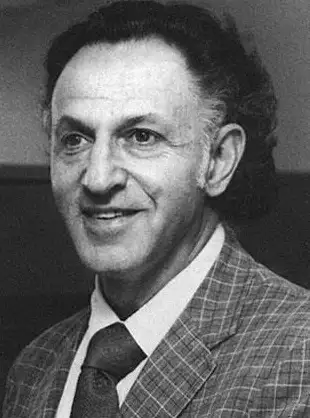
\includegraphics[clip, width = 2.0cm]{Bellman.png}\\
                            {\tiny Bellman}
                            \centering
                        \end{column}
                        \begin{column}{.5\textwidth}
                            Bellman方程式 \\
                            HJB方程式 \\
                        \end{column}
                    \end{columns}
                \end{boxnote}
            \end{column}

            \begin{column}{0.5\textwidth}
                \begin{boxnote}
                    \begin{columns}
                        \begin{column}{.5\textwidth}
                            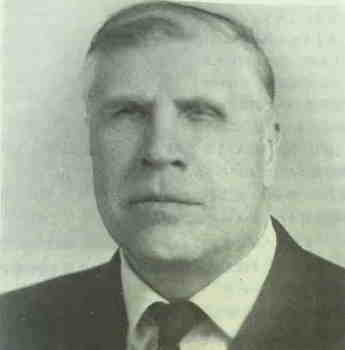
\includegraphics[clip, width = 2.0cm]{Pontryagin.png}\\
                            {\tiny Pontryagin}
                            \centering
                        \end{column}
                        \begin{column}{.5\textwidth}
                            最小原理 \\
                        \end{column}
                    \end{columns}
                \end{boxnote}
            \end{column}
        \end{columns}

    \end{frame}

    \begin{frame}{現在位置}
        \footnotesize
        \begin{columns}
            \begin{column}{.35\textwidth}
                \begin{itemize}
                    \item 復習
                    \item \colorbox{yellow}{動的計画法}
                    \item HJB方程式
                    \item 最小原理
                    \item MPC導入
                \end{itemize}
            \end{column}
    
            \begin{column}{.7\textwidth}
                線形MPCでは離散状態を考えたけど、連続での制御を考える \\
                \fontsize{6.5pt}{3.5pt}\selectfont
                \begin{tcolorbox}[title=Bellman方程式]
                    \begin{equation*}
                        V(x, t) = \min_{u[t, t+dt]} \left( L(x, u, t) dt + V \left( x + f(x, u, t) dt, t + dt \right) \right)
                    \end{equation*}
                \end{tcolorbox}
                
            \end{column}
        \end{columns}
    \end{frame}

    \begin{frame}{動的計画法1}
        \footnotesize
        \begin{tcolorbox}[title=最適制御]
            状態方程式 \quad $\dot{x}(t) = f(x(t), u(t), t)$ \\
            評価関数 \qquad $J =$ 
            \tikz[remember picture, baseline=(T1.base)]{
                \node [fill=orange!20!white, inner sep=0pt, outer sep=0, minimum height=4ex] (T1) {$\phi(x(t_f))$};
            }
            $+$
            \tikz[remember picture, baseline=(T2.base)]{
                \node [fill=red!20!white, inner sep=0pt, outer sep=0, minimum height=4ex] (T2) {$\int_{t_0}^{t_f} L(x(t), u(t), t) \, dt$}
            }
             
            \begin{tikzpicture}[remember picture, overlay]
              \node [below=0pt of T1, text=orange!80!black] {終端コスト};
              \node [below=0pt of T2, text=red!80!black] {ステージコスト};
            \end{tikzpicture}

        \end{tcolorbox}
    
        \textcolor{blue}{価値関数$V(x, t)$}:評価関数$J$を最小にする値\\
        \begin{align*}
            \textcolor{blue}{V(x, t)} = \min_{u[t, t_f]} \left( \phi(x(t_f)) + \int_t^{t_f} L(x(\tau), u(\tau), \tau) d\tau \right)
        \end{align*}
        最適化を\textcolor{blue}{価値関数}を探すことだと考える
    
    \end{frame}

    \begin{frame}{動的計画法2}
        
        \begin{columns}
            \begin{column}{.5\textwidth}
                \begin{tikzpicture}
                    \draw[->, >=stealth, semithick](-0.5, 0)--(3.5, 0)node[right]{$x$};
                    \draw[->, >=stealth, semithick](0, -0.5)--(0, 3.5)node[above]{$y$};
                    \draw[dashed](1, -0.5)node[below]{$t_0$}--(1, 3.5);
                    \draw[dashed](3, -0.5)node[below]{$t_f$}--(3, 3.5);
                \end{tikzpicture}
            \end{column}

            \begin{column}{.5\textwidth}
                \begin{tikzpicture}
                    \coordinate(A)at(0, 0);
                    \coordinate(B)at(1, 0);
                    \draw[->](A)--(B);
                    \draw(A)node[left]{$t_0$};
                    \draw(B)node[right]{$t_f$};
                \end{tikzpicture}

                \begin{tikzpicture}
                    \coordinate(A)at(0, 0);
                    \coordinate(B)at(0.5, 0);
                    \draw[->](A)--(B);
                    \draw(A)node[left]{$t_0$};
                    \draw(B)node[right]{$t_0+dt$};

                    \coordinate(C)at(4.0, 0);
                    \coordinate(D)at(4.5, 0);
                    \draw[->](C)--(D);
                    \draw(C)node[left]{$t_0+dt$};
                    \draw(D)node[right]{$t_f$};
                \end{tikzpicture}
            \end{column}
        \end{columns}
    \end{frame}
    
    \begin{frame}{動的計画法3}
        \scriptsize
        \fontsize{6.5pt}{6.5pt}\selectfont

        \begin{align*}
            V(x, t) &= \min_{u[t, t_f]} \left( \phi(x(t_f)) + \int_t^{t_f} L(x(\tau), u(\tau), \tau) d\tau \right) \\
            &= \min_{u[t, t_f]} \left( \int_t^{t+dt} L(x(\tau), u(\tau), \tau) d\tau + \colorbox{yellow}{$\phi(x(t_f)) + \int_{t+dt}^{t_f} L(x(\tau), u(\tau), \tau) d\tau$} \right) \\
            &= \min_{u[t, t+dt]} \left( \int_t^{t+dt} L(x(\tau), u(\tau), \tau) d\tau + \min_{u[t+dt, t_f]} \left( \phi(x(t_f)) + \int_{t+dt}^{t_f} L(x(\tau), u(\tau), \tau) d\tau \right) \right) \\
            &= \min_{u[t, t+dt]} \left( \int_t^{t+dt} L(x(\tau), u(\tau), \tau) d\tau + V \left( x + \int_t^{t+dt} f(x, u, \tau) d\tau, t + dt \right) \right) \\
        \end{align*}

        \begin{tcolorbox}[title=Bellman方程式]
            \begin{align*}
                &V(x, t) &=& \min_{u[t, t+dt]} \left( L(x, u, t) dt + V \left( x + f(x, u, t) dt, t + dt \right) \right) \\
                &V(x, t_f) &=& \phi(x(t_f))
            \end{align*}
        \end{tcolorbox}

        Bellman方程式が解ければ最適制御ができる!!!(もともとの評価関数を満たす解を求めるのと一緒) \\
        目標の状態$x(t_f)$が分かっていれば解けそう?? \\
    \end{frame}

    \begin{frame}{動的計画法4}
        \footnotesize
        \begin{tcolorbox}[title=Bellman方程式]
            \begin{align*}
                V(x, t) &= \min_{u[t, t+dt]} \left( L(x, u, t) dt + V \left( x + f(x, u, t) dt, t + dt \right) \right)
            \end{align*}
        \end{tcolorbox}
        \begin{tcolorbox}[title=次元の呪い]
            次元の呪いは、状態空間や行動空間の次元数が増加するにつれて、必要な計算量やメモリが指数的に増加する現象 \\
            2次元の格子が10の場合、合計100のセルが存在します。しかし、10次元の格子が各次元に10のセルを持つ場合、合計で$10^10 = 10,000,000,000$のセルが存在します。このように、次元が増加するにつれて格子の数が指数的に増加し、それに伴い計算量も指数的に増加します。
        \end{tcolorbox}
        次元の呪いのグラフを貼る \\
        \centering
    \end{frame}

    \begin{frame}{動的計画法まとめ}
        動的計画法は大きな問題を小さな部分問題に分解し、それぞれ解くことで全体の解を得る手法

        \begin{tcolorbox}[title=Bellman方程式]
            \begin{align*}
                V(x, t) &= \min_{u[t, t+dt]} \left( L(x, u, t) dt + V \left( x + f(x, u, t) dt, t + dt \right) \right)
            \end{align*}
        \end{tcolorbox}

        \begin{itemize}
            \item 最適的な性質を持つ
            \item 計算結果を保存して再利用(メモ化)
        \end{itemize}
    \end{frame}

    \begin{frame}{現在位置}
        \footnotesize
        \begin{itemize}
            \item 復習
            \item 動的計画法
            \item \colorbox{yellow}{HJB方程式}
            \item 最小原理
            \item MPC導入
        \end{itemize}
        \begin{itembox}[l]{Bellman方程式からHJB方程式への変形}
            \begin{align*}
                V(x, t) &= \min_u \left( L(x, u, t) dt + V \left( x + f(x, u, t) dt, t + dt \right) \right)        
            \end{align*}
            \begin{align*}
                -\frac{\partial V}{\partial t}\left(x,t\right) = \min _u H\left(x, u, \left( \frac{\partial V}{\partial x} \right)^T\left(x, t\right), t \right)
            \end{align*}
        \end{itembox}
    \end{frame}

    \begin{frame}{HJB方程式}
        \fontsize{6.5pt}{6.5pt}\selectfont

        \colorbox{yellow}{$V(x, t) = \min_{u} \left( L(x, u, t) dt + V \left( x + f(x, u, t) dt, t + dt \right) \right)$} \\
        
        $V \left( x + f(x, u, t) dt, t + dt \right)$を$(x, t)$でTaylor展開する\\
        \begin{equation*}
            V \left( x + f(x, u, t) dt, t + dt \right) \simeq V \left(x, t\right) + \frac{\partial V}{\partial x}\left(x, t\right)f\left(x, u, t\right)dt + \frac{\partial V}{\partial t}\left(x, t\right)dt
        \end{equation*}
 
        
        \begin{align*}
            V(x, t) &= \min_{u[t, t+dt]} \left( L(x, u, t) dt + V \left(x, t\right) + \frac{\partial V}{\partial x}\left(x, t\right)f\left(x, u, t\right)dt + \frac{\partial V}{\partial t}\left(x, t\right)dt \right) \\
            0&=\min_{u[t, t+dt]} \left( L(x, u, t) dt + \frac{\partial V}{\partial x}\left(x, t\right)f\left(x, u, t\right)dt + \frac{\partial V}{\partial t}\left(x, t\right)dt \right) \\
            H(x, u, \lambda, t) &= L(x, u, t) + \lambda^T f(x, u, t) \\
            H\left(x, u, \left( \frac{\partial V}{\partial x} \right)^T\left(x, t\right), t \right) &= L(x, u, t) + \frac{\partial V}{\partial x}\left(x, t\right)f\left(x, u, t\right) \\
        \end{align*}

        \colorbox{yellow}{$-\frac{\partial V}{\partial t}\left(x,t\right) = \min _u H\left(x, u, \left( \frac{\partial V}{\partial x} \right)^T\left(x, t\right), t \right)$} \\

    \end{frame}

    \begin{frame}{現在位置}
        \footnotesize
        \begin{itemize}
            \item 復習
            \item 動的計画法
            \item HJB方程式
            \item \colorbox{yellow}{最小原理}
            \item MPC導入
        \end{itemize}
        別の観点から最適制御を考える \\
        \begin{figure}[H]
            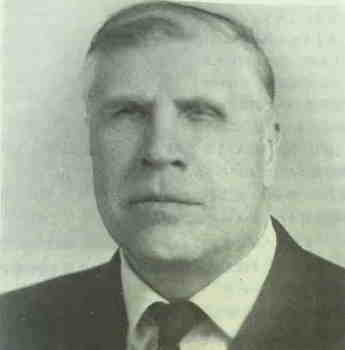
\includegraphics[clip, width = 2.0cm]{Pontryagin.png}
        \end{figure}
        \tiny{
            \rightline{
                Pontryagin
            }
        }
    \end{frame}

    \begin{frame}{最小原理1}
        \footnotesize

    \end{frame}

    \begin{frame}{最小原理2}
        \footnotesize
        もちろん最小原理からHJB方程式を導ける

    \end{frame}

    \begin{frame}{最適性条件まとめ}
        \footnotesize
        ラグランジュの未定乗数法\\
        KKT条件\\
        オイラーラグランジュ方程式\\
        動的計画法(new)\\
        HJB方程式(new)\\
        最小原理(new)\\
        動的計画法からHJB方程式を導いたが、最小原理からも導ける\\

        ここに各関係の図を貼る
    \end{frame}
    \begin{frame}{現在位置}
        \footnotesize
        \begin{itemize}
            \item 復習
            \item 動的計画法
            \item HJB方程式
            \item 最小原理
            \item \colorbox{yellow}{MPC導入}
        \end{itemize}
    \end{frame}

    \begin{frame}{MPC}
        Euler-Lagrange方程式では入力に状態を含んでいないので、状態が変化(外的要因によって)する現実システムだと扱いにくい \\
        HJB方程式は入力に状態を含んでいるが、偏微分方程式なので扱いにくい \\
        現実問題に落とし込んだのがMPC \\
        評価区間が無限のMPCの解はHJB方程式と一致するはず(たぶん...) \\
    \end{frame}

    \begin{frame}{参考資料}
        \footnotesize

        書籍\\
        \begin{itemize}
            \item 非線形最適制御入門(名著です)
            \item しっかり学ぶ数理最適化(最適化全般について)
            \item はじめての最適化(変分法の説明が分かりやすいです)
        \end{itemize}
    \end{frame}
    
\end{document}